% UICTEST.TEX
% This is a test file for my port of UICTHESI
% to LaTeX 2e. This is based in part on UCTHESIS.
%

\documentclass{uicthesi}




\usepackage{booktabs} % For formal tables

\usepackage{framed}
\usepackage{hyperref}
\usepackage{balance}
\usepackage[dvips]{graphics,color}

\usepackage{epsfig}
\usepackage{color}
\usepackage{subfigure}
\usepackage{multirow,tabularx}
\usepackage{placeins}
%\usepackage{miniltx}
\usepackage{mathtools}
\usepackage{graphicx}
\usepackage{epstopdf}
\usepackage{bm}

\usepackage{csquotes}
\usepackage{array}
\usepackage[yyyymmdd,hhmmss]{datetime}
\usepackage[subject={Todo}]{pdfcomment}
\usepackage[textsize=scriptsize,bordercolor=black!20]{todonotes}
\usepackage{xcolor,colortbl}
\usepackage{amssymb}% http://ctan.org/pkg/amssymb
\usepackage{pifont}% http://ctan.org/pkg/pifont
\usepackage[algo2e,titlenumbered,ruled]{algorithm2e} 
\usepackage{lipsum,environ,amsmath}
\usepackage{slashbox,booktabs,amsmath}
%\usepackage{todonotes}
\usepackage{cite}

\usepackage{xspace}

\hyphenation{PageRank Convex dictatorship Dic-ta-tor-ship}

\newcounter{Lcount}
\newcommand{\numsquishlist}{
   \begin{list}{\arabic{Lcount}. }
    { \usecounter{Lcount}
 \setlength{\itemsep}{-.1ex}      \setlength{\parsep}{0ex}
      \setlength{\topsep}{0ex}       \setlength{\partopsep}{0ex}
      \setlength{\leftmargin}{1em} \setlength{\labelwidth}{1em}
      \setlength{\labelsep}{0.1em} } }
\newcommand{\numsquishend}{\end{list}}

\newcommand{\squishlist}{
   \begin{list}{$\bullet$}
    { \setlength{\itemsep}{-.1ex}      \setlength{\parsep}{0ex}
      \setlength{\topsep}{0ex}       \setlength{\partopsep}{0ex}
      \setlength{\leftmargin}{.8em} \setlength{\labelwidth}{1em}
      \setlength{\labelsep}{0.5em} } }
\newcommand{\squishend}{\end{list}}



\makeatletter
\DeclareOldFontCommand{\rm}{\normalfont\rmfamily}{\mathrm}
\DeclareOldFontCommand{\sf}{\normalfont\sffamily}{\mathsf}
\DeclareOldFontCommand{\tt}{\normalfont\ttfamily}{\mathtt}
\DeclareOldFontCommand{\bf}{\normalfont\bfseries}{\mathbf}
\DeclareOldFontCommand{\it}{\normalfont\itshape}{\mathit}
\DeclareOldFontCommand{\sl}{\normalfont\slshape}{\@nomath\sl}
\DeclareOldFontCommand{\sc}{\normalfont\scshape}{\@nomath\sc}
\makeatother


\newcounter{problem}
\newenvironment{problem}[1][htb]
  {\renewcommand{\algorithmcfname}{Problem}% Update algorithm name
   \begin{algorithm2e}[#1]%
   \SetAlFnt{\small}
    \SetAlCapFnt{\small}
    \SetAlCapNameFnt{\small}
    \SetAlCapHSkip{0pt}
  }{\end{algorithm2e}}
  
  \newenvironment{alprocedure}[1][htb]
  {\renewcommand{\algorithmcfname}{Procedure}% Update algorithm name
   \begin{algorithm2e}[#1]%
    \SetAlFnt{\small}
\SetAlCapFnt{\small}
\SetAlCapNameFnt{\small}
\SetAlCapHSkip{0pt}
\IncMargin{-\parindent}
   
  }{\end{algorithm2e}}
  


\begin{document}

% Declarations for Front Matter

\title{Title of Thesis is here}
\author{First-name Lastname}
\pdegrees{}
\degree{Doctor of Philosophy in Computer Science}
\committee{Prof. Firstname1 Lastname1, Chair and Advisor \\ Prof. Firstname2 Lastname2  \\ Prof. Firstname3 Lastname3 \\ Prof. Firstname4 Lastname4 \\ Prof. Firstname5 Lastname5}
\maketitle


% \dedication
% {\null\vfil
% {\large
% \begin{center}
% To myself,\\\vspace{12pt}
% Perry H. Disdainful,\\\vspace{12pt}
% the only person worthy of my company.
% \end{center}}
% \vfil\null}


 \acknowledgements
{The thesis has been completed... (INSERT YOUR TEXTS)\\ 

\begin{flushright}YOUR INITIAL\end{flushright}}
% \acknowledgements
% {I want to ``thank'' my committee, without whose ridiculous demands, I
% would have graduated so, so, very much faster.}

% \preface
% This preface is purely optional at UIC.

\tableofcontents
\listoftables
\listoffigures
\listofabbreviations
\begin{list}
{}
{\setlength
  {\labelwidth}{1in}
    \setlength{\leftmargin}{1.5in}
    \setlength{\labelsep}{.5in}
    \setlength{\rightmargin}{\leftmargin}}
\item[AMS\hfill] American Mathematical Society
\item[CTAN\hfill] Comprehensive \TeX\ Archive Network
\item[TUG\hfill] \TeX\ Users Group
\item[UIC\hfill] University of Illinois at Chicago
\item[UICTHESI\hfill] Thesis formatting system for use at UIC.
\end{list}
 
\summary
Put your summary of thesis here.

\chapter{Introduction}

This is how we cite a paper \cite{Farine20162243}.

Below is the example of algorithm block.


\IncMargin{1em}
\begin{alprocedure}[!htp]
\caption{FindFactionsAndInitiators}
\SetKwInOut{Input}{input}\SetKwInOut{Output}{output}
\Input{An adjacency matrix $E^*$ of dynamic network}
\Output{ A time series of faction sets $\mathcal{F}^*$, and a time series of initiator sets $\mathcal{L}^*$ }
\BlankLine
\For{$i\leftarrow 1$ \KwTo $t^*$}{
\textcolor{cyan}{\tcc*[h]{Get a matrix at time $t=i$} }

$E \leftarrow E^*_{ t = i}$ \; 
\textcolor{cyan}{\tcc*[h]{FindInitiators($E $) returns all nodes which have zero outgoing degree}}

$\mathcal{L} \leftarrow$FindInitiators($E $) \;
$\mathcal{F} = \emptyset$ \;
\For{$l \in \mathcal{L}$}{
\textcolor{cyan}{\tcc*[h]{FindReachNodeFrom($E,l$) returns all nodes which have any directed path to $l$}}

$F_l\leftarrow$FindReachNodeFrom($E,l$) \;
$\mathcal{F} = \mathcal{F} \cup \{F_l\}$
}
$\mathcal{F}^*_{t=i} = \mathcal{F}  $ and $\mathcal{L}^*_{t=i} = \mathcal{L}  $
}
\label{algo:FindFactionsAndInitiators}
\end{alprocedure}\DecMargin{1em}


The example of table is below.

\begin{table}[!htp]
\tiny
\centering
\caption{Table Caption1}
\label{table:htestdes}
\begin{tabular}{l|l|l|}
\cline{2-3}
                                                                                                                     & \cellcolor[HTML]{EFEFEF}\textbf{Method}                                    & \cellcolor[HTML]{EFEFEF}\textbf{Null hypothesis $H_0$}                                                                                          \\ \hline
\multicolumn{1}{|l|}{}                                                                                               & $t$-test                                                                      & \begin{tabular}[c]{@{}l@{}}A sample has a normal distribution \\ with zero mean and unknown variance.\end{tabular}                              \\ \cline{2-3} 
\multicolumn{1}{|l|}{}                                                                                               & \cellcolor[HTML]{EFEFEF}Sign test                                          & \cellcolor[HTML]{EFEFEF}A sample has a distribution with zero median.                                                                           \\ \cline{2-3} 
\multicolumn{1}{|l|}{\multirow{-3}{*}{\textbf{\begin{tabular}[c]{@{}l@{}}Zero \\ mean/median \\ test\end{tabular}}}} & Wilcoxon signed rank test                                                  & A sample has a symmetric distribution around zero median.                                                                                       \\ \hline
\multicolumn{1}{|l|}{}                                                                                               & \cellcolor[HTML]{EFEFEF}Kolmogorov-Smirnov test (KS test)                           & \cellcolor[HTML]{EFEFEF}A sample comes from a normal distribution.                                                                              \\ \cline{2-3} 
\multicolumn{1}{|l|}{}                                                                                               & \begin{tabular}[c]{@{}l@{}}Chi-square \\ goodness-of-fit test\end{tabular} & \begin{tabular}[c]{@{}l@{}}A sample comes from a normal distribution \\ with a mean and variance estimated from a sample itself.\end{tabular}   \\ \cline{2-3} 
\multicolumn{1}{|l|}{}                                                                                               & \cellcolor[HTML]{EFEFEF}Jarque-Bera test                                   & \cellcolor[HTML]{EFEFEF}\begin{tabular}[c]{@{}l@{}}A sample comes from a normal distribution \\ with an unknown mean and variance.\end{tabular} \\ \cline{2-3} 
\multicolumn{1}{|l|}{\multirow{-4}{*}{\textbf{\begin{tabular}[c]{@{}l@{}}Normality \\ test\end{tabular}}}}           & Anderson-Darling test                                                      & A sample comes from a normal distribution.                                                                                                      \\ \hline
\end{tabular}
\end{table}



\section{Support of leading faction}

\begin{figure}[ht!]
\centering
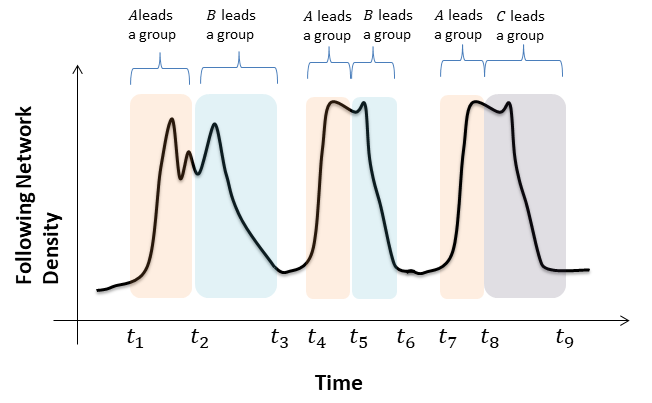
\includegraphics[width=0.9\columnwidth]{FIG/CoorEventSup}
\caption{An example of image in thesis }
\label{fig:CoorEventSup}
\end{figure}


 \appendices
 \newpage
 \appendix

 \chapter{Some Ancillary Stuff}

 Ancillary material should be put in appendices.

 \chapter{Some More Ancillary Stuff}

% Here is yet another appendix! Wahoo!

%\nocite{*}
\bibformb
\bibliography{BibFile}
\newpage
% \vita
% This is where the vita goes.  Its organization is left as an exercise.
\clearpage
    \pagestyle{pageontop}
   \thispagestyle{pageonbottom}
   %\vspace*{3in}
   \begin{large}
   \begin{center}
   {\bfseries VITA}
   \end{center}
   \end{large}
\begin{tabular}{p{2.8cm}p{10.5cm}}
NAME: & NAME LASTNAME  \\ 
    &\\
EDUCATION:  &Ph.D., Computer Science, University of Illinois at Chicago, Chicago, Illinois, 2018. \\  
            &\\
            &M.Eng., Computer Engineering, University of Illinois at Chicago, Chicago, Illinois, 20xx.\\
            &\\
            &B.Eng., Computer Engineering, University of Illinois at Chicago, Chicago, Illinois, 20xx.  \\
            &\\
ACADEMIC EXPERIENCE:  &Research Assistant, Computational Population Biology Lab, Department of Computer Science, University of Illinois at Chicago, xxxx - 2018. \\
            &\\
            &Teaching Assistant, Department of Computer Science, University of Illinois at Chicago: \\
            &\squishlist            
            \item Computer Algorithm I, Spring xxxx and  Fall xxxx.    
            \item Secure Computer Systems, Fall xxxx 
            \squishend \\
            

 \end{tabular}

\end{document}
